% \VignetteIndexEntry{Cell Ranger R Kit Tutorial: Secondary Analysis on 10x Single Cell 3' RNA-seq PBMC Data}
% \VignetteEngine{knitr::knitr}
% \VignetteDepends{}
% \VignettePackage{cellrangerrkit}

%
% Copyright (c) 2016 10x Genomics, Inc. All rights reserved.
%

\documentclass[10pt,oneside]{article}\usepackage[]{graphicx}\usepackage[]{color}
%% maxwidth is the original width if it is less than linewidth
%% otherwise use linewidth (to make sure the graphics do not exceed the margin)
\makeatletter
\def\maxwidth{ %
  \ifdim\Gin@nat@width>\linewidth
    \linewidth
  \else
    \Gin@nat@width
  \fi
}
\makeatother

\definecolor{fgcolor}{rgb}{0.345, 0.345, 0.345}
\newcommand{\hlnum}[1]{\textcolor[rgb]{0.686,0.059,0.569}{#1}}%
\newcommand{\hlstr}[1]{\textcolor[rgb]{0.192,0.494,0.8}{#1}}%
\newcommand{\hlcom}[1]{\textcolor[rgb]{0.678,0.584,0.686}{\textit{#1}}}%
\newcommand{\hlopt}[1]{\textcolor[rgb]{0,0,0}{#1}}%
\newcommand{\hlstd}[1]{\textcolor[rgb]{0.345,0.345,0.345}{#1}}%
\newcommand{\hlkwa}[1]{\textcolor[rgb]{0.161,0.373,0.58}{\textbf{#1}}}%
\newcommand{\hlkwb}[1]{\textcolor[rgb]{0.69,0.353,0.396}{#1}}%
\newcommand{\hlkwc}[1]{\textcolor[rgb]{0.333,0.667,0.333}{#1}}%
\newcommand{\hlkwd}[1]{\textcolor[rgb]{0.737,0.353,0.396}{\textbf{#1}}}%

\usepackage{framed}
\makeatletter
\newenvironment{kframe}{%
 \def\at@end@of@kframe{}%
 \ifinner\ifhmode%
  \def\at@end@of@kframe{\end{minipage}}%
  \begin{minipage}{\columnwidth}%
 \fi\fi%
 \def\FrameCommand##1{\hskip\@totalleftmargin \hskip-\fboxsep
 \colorbox{shadecolor}{##1}\hskip-\fboxsep
     % There is no \\@totalrightmargin, so:
     \hskip-\linewidth \hskip-\@totalleftmargin \hskip\columnwidth}%
 \MakeFramed {\advance\hsize-\width
   \@totalleftmargin\z@ \linewidth\hsize
   \@setminipage}}%
 {\par\unskip\endMakeFramed%
 \at@end@of@kframe}
\makeatother

\definecolor{shadecolor}{rgb}{.97, .97, .97}
\definecolor{messagecolor}{rgb}{0, 0, 0}
\definecolor{warningcolor}{rgb}{1, 0, 1}
\definecolor{errorcolor}{rgb}{1, 0, 0}
\newenvironment{knitrout}{}{} % an empty environment to be redefined in TeX

\usepackage{alltt}

\newcommand{\tm}{\textsuperscript{\tiny	{TM}}~}
\newcommand{\weblink}[1]{\newline \newline {\color{Violet}{\texttt{~ #1}}} \newline \newline}

% \newcommand{\weblink}[1]{ {\color{Violet}\verb!#1! }}
% \newcommand{\weblink}[1]{\begin{verbatim}#1\end{verbatim}}
% \newcommand{\weblink}[1]{{\color{Violet}\begin{verbatim}#1\end{verbatim}}}

\newcommand{\thetitle}{Cell Ranger\textsuperscript{\footnotesize {TM}} R Kit Tutorial: Secondary Analysis on \\ 10x Genomics\textsuperscript{\footnotesize	{TM}} Single Cell 3' RNA-seq PBMC Data}


\usepackage{whbiocvignette}
\usepackage{listings}
\usepackage{hyperref}
\usepackage[usenames,dvipsnames]{xcolor}
\usepackage{fancyhdr}

% Turn on the style
\pagestyle{fancy}
\fancyhead{}
\fancyfoot{}
\fancyfoot[C]{\thepage}


\title{\textsf{\textbf{\thetitle}}}
\author{10x Genomics\tm}
\IfFileExists{upquote.sty}{\usepackage{upquote}}{}
\begin{document}

\maketitle

% \begin{abstract}
% \end{abstract}

\tableofcontents


\vspace{0.5in}
\section{Introduction}
\subsection{Overview of this tutorial}
This tutorial provides instructions on how to perform exploratory secondary analysis on single cell 3' RNA-seq data produced by the 10x Genomics\tm Chromium\tm Platform, and processed by the Cell Ranger\tm pipeline. We illustrate an example workflow using peripheral blood mononuclear cells (PBMCs) from a healthy donor, using two data sets: \verb!pbmc3k! and \verb!pbmc6k! (from the same donor) released by 10x Genomics\tm:
{\color{Violet}
\begin{verbatim}
  http://support.10xgenomics.com/single-cell/datasets/pbmc3k
  http://support.10xgenomics.com/single-cell/datasets/pbmc6k
\end{verbatim}}
\noindent
In this tutorial, you will learn how to:
\begin{itemize}
\item
Load processed data from the Cell Ranger\tm pipeline or public data provided by 10x Genomics\tm
\item
Perform unsupervised clustering for {\it de novo} cell-type discovery
\item
Visualize clustering of single cells and cluster-specific gene expression signatures
\item
Combine data from multiple experiments
\end{itemize}
\subsection{Additional resources}
You can learn more about the Cell Ranger\tm pipeline here:
\weblink{http://support.10xgenomics.com/single-cell/software/pipelines/latest/what-is-cell-ranger}
A larger number of other publicly available single cell data sets released by 10x Genomics\tm are available here:
\weblink{http://support.10xgenomics.com/single-cell/datasets}
If you have any questions about the data and the analysis, please contact {\bf \verb!support@10xgenomics.com!}.

\vspace{0.5in}

\section{Getting Started}
\subsection{Installing Cell Ranger R Kit}
You can follow the instructions at the link below to install R Kit and its dependencies:
\weblink{http://support.10xgenomics.com/single-cell/software/pipelines/latest/rkit}
\subsection{Loading gene expression data for secondary analysis}
The Chromium\tm Cell Ranger\tm pipeline produces processed gene-barcode matrices and primary results. By specifiying the pipeline output directory (or {\it pipestance path}), you can use the R kit to load these pipeline results into your local R environment. You can load the pipeline data by specifying a pipestance path in R as follows.
\begin{knitrout}
\definecolor{shadecolor}{rgb}{0.969, 0.969, 0.969}\color{fgcolor}\begin{kframe}
\begin{alltt}
\hlstd{cellranger_pipestance_path} \hlkwb{<-} \hlstr{"/path/to/your/pipeline/output/directory"}
\hlstd{gbm} \hlkwb{<-} \hlkwd{load_cellranger_matrix}\hlstd{(cellranger_pipestance_path)}
\hlstd{analysis_results} \hlkwb{<-} \hlkwd{load_cellranger_analysis_results}\hlstd{(cellranger_pipestance_path)}
\end{alltt}
\end{kframe}
\end{knitrout}
\noindent
Alternatively, you can download the publicly available data to a local path using the \verb!download_sample! function and treat this local path as your pipestance path.
\begin{knitrout}
\definecolor{shadecolor}{rgb}{0.969, 0.969, 0.969}\color{fgcolor}\begin{kframe}
\begin{alltt}
\hlstd{pipestance_path} \hlkwb{<-} \hlstr{"/path/to/your/local/directory/for/pbmc3k"}
\hlkwd{download_sample}\hlstd{(}\hlkwc{sample_name}\hlstd{=}\hlstr{"pbmc3k"}\hlstd{,}\hlkwc{sample_dir}\hlstd{=pipestance_path,}
                \hlkwc{host}\hlstd{=}\hlstr{"https://s3-us-west-2.amazonaws.com/10x.files/samples/cell/"}\hlstd{)}
\hlstd{gbm} \hlkwb{<-} \hlkwd{load_cellranger_matrix}\hlstd{(pipestance_path)}
\hlstd{analysis_results} \hlkwb{<-} \hlkwd{load_cellranger_analysis_results}\hlstd{(pipestance_path)}
\end{alltt}
\end{kframe}
\end{knitrout}

The variable \verb!gbm! is an object based on the Bioconductor ExpressionSet class that stores the barcode filtered gene expression matrix and metadata, such as gene symbols and barcode IDs corresponding to cells in the data set. The gene expression values, gene information and cell barcodes can be accessed using:
\begin{knitrout}
\definecolor{shadecolor}{rgb}{0.969, 0.969, 0.969}\color{fgcolor}\begin{kframe}
\begin{alltt}
\hlkwd{exprs}\hlstd{(gbm)} \hlcom{# expression matrix}
\hlkwd{fData}\hlstd{(gbm)} \hlcom{# data frame of genes}
\hlkwd{pData}\hlstd{(gbm)} \hlcom{# data frame of cell barcodes}
\end{alltt}
\end{kframe}
\end{knitrout}
The variable \verb!analysis_results! contains pre-computed results for principle component analysis (PCA) dimensional reduction, t-SNE (t-Distributed Stochastic Neighbor Embedding) projection, and k-means clustering. Because each cell is represented by a high-dimensional gene expression profile, one way to visualize cell-to-cell similarity is by reducing the data set to a two dimensional representation. There are many dimension reduction methods available for 2-D visualization. Here we include implementations of two popular approaches, PCA and t-SNE, with pre-computed results stored in \verb!analysis_results!.

For instance, you can access the t-SNE projection and plot the cells colored by UMI counts as follows.

\begin{figure}[htbp]
\begin{center}
\begin{knitrout}
\definecolor{shadecolor}{rgb}{0.969, 0.969, 0.969}\color{fgcolor}\begin{kframe}
\begin{alltt}
\hlstd{tsne_proj} \hlkwb{<-} \hlstd{analysis_results}\hlopt{$}\hlstd{tsne}
\hlkwd{visualize_umi_counts}\hlstd{(gbm,tsne_proj[}\hlkwd{c}\hlstd{(}\hlstr{"TSNE.1"}\hlstd{,}\hlstr{"TSNE.2"}\hlstd{)],}\hlkwc{limits}\hlstd{=}\hlkwd{c}\hlstd{(}\hlnum{3}\hlstd{,}\hlnum{4}\hlstd{),}\hlkwc{marker_size}\hlstd{=}\hlnum{0.05}\hlstd{)}
\end{alltt}
\end{kframe}

{\centering 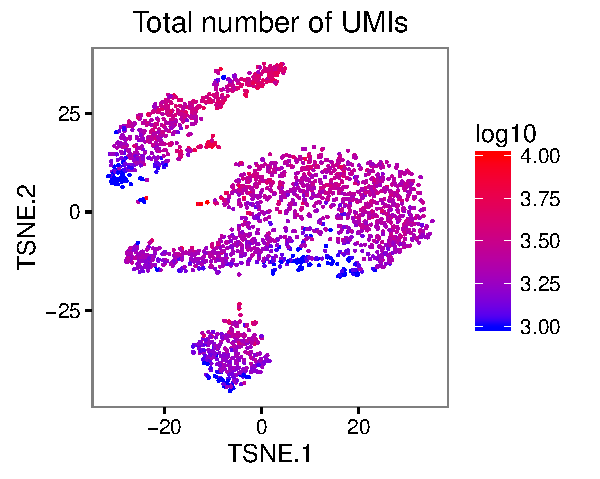
\includegraphics[width=\maxwidth]{figure/umi-1} 

}



\end{knitrout}
\caption{t-SNE projection where each cell is colored by log10 of UMI counts. Color scale represents log10 of UMI counts.}
\label{fig:umi}
\end{center}
\end{figure}

\vspace{0.3in}

Each point in the scatter plot represents a cell in the coordinates specified by the two t-SNE components. The color of each point plotted by \verb!visualize_umi_counts! (Figure \ref{fig:umi}) indicates the total number of UMIs for each cell, and these count values are displayed in log10 scale.

Cells with similar expression profile tend to appear closer in the 2-D space, so you may already see some structures in the data. However, to identify what the structures represent, you will need to rely on the gene signatures that each cell expresses to draw meaningful insights from the data. Instead of using raw UMI counts for downstream differential gene analysis, we recommend that you filter unexpressed genes, normalize the UMI counts for each barcode, and use the log-transformed gene-barcode matrix. After transformation, the gene-barcode matrix contains 16634 genes for 2700 cells.
\begin{knitrout}
\definecolor{shadecolor}{rgb}{0.969, 0.969, 0.969}\color{fgcolor}\begin{kframe}
\begin{alltt}
\hlstd{use_genes} \hlkwb{<-} \hlkwd{get_nonzero_genes}\hlstd{(gbm)}
\hlstd{gbm_bcnorm} \hlkwb{<-} \hlkwd{normalize_barcode_sums_to_median}\hlstd{(gbm[use_genes,])}
\hlstd{gbm_log} \hlkwb{<-} \hlkwd{log_gene_bc_matrix}\hlstd{(gbm_bcnorm,}\hlkwc{base}\hlstd{=}\hlnum{10}\hlstd{)}
\hlkwd{print}\hlstd{(}\hlkwd{dim}\hlstd{(gbm_log))}
\end{alltt}
\begin{verbatim}
## [1] 16634  2700
\end{verbatim}
\end{kframe}
\end{knitrout}

\vspace{0.5in}
\section{Visualizing signatures of known gene markers}
One way to identify different cell types is by expression of specific genes in cells. You can visualize expression values of a set of genes to identify cells where particular genes are up-regulated. Here, we show how to simultaneously plot the expression of 6 gene markers, one for each subplot using the \verb!visualize_gene_markers! function.

\begin{figure}[htbp]
\begin{center}
\begin{knitrout}
\definecolor{shadecolor}{rgb}{0.969, 0.969, 0.969}\color{fgcolor}\begin{kframe}
\begin{alltt}
\hlstd{genes} \hlkwb{<-} \hlkwd{c}\hlstd{(}\hlstr{"CD79A"}\hlstd{,}\hlstr{"NKG7"}\hlstd{,}\hlstr{"CD3D"}\hlstd{,}\hlstr{"CST3"}\hlstd{,}\hlstr{"CD8A"}\hlstd{,}\hlstr{"PF4"}\hlstd{)}
\hlstd{tsne_proj} \hlkwb{<-} \hlstd{analysis_results}\hlopt{$}\hlstd{tsne}
\hlkwd{visualize_gene_markers}\hlstd{(gbm_log,genes,tsne_proj[}\hlkwd{c}\hlstd{(}\hlstr{"TSNE.1"}\hlstd{,}\hlstr{"TSNE.2"}\hlstd{)],}\hlkwc{limits}\hlstd{=}\hlkwd{c}\hlstd{(}\hlnum{0}\hlstd{,}\hlnum{1.5}\hlstd{))}
\end{alltt}
\end{kframe}

{\centering 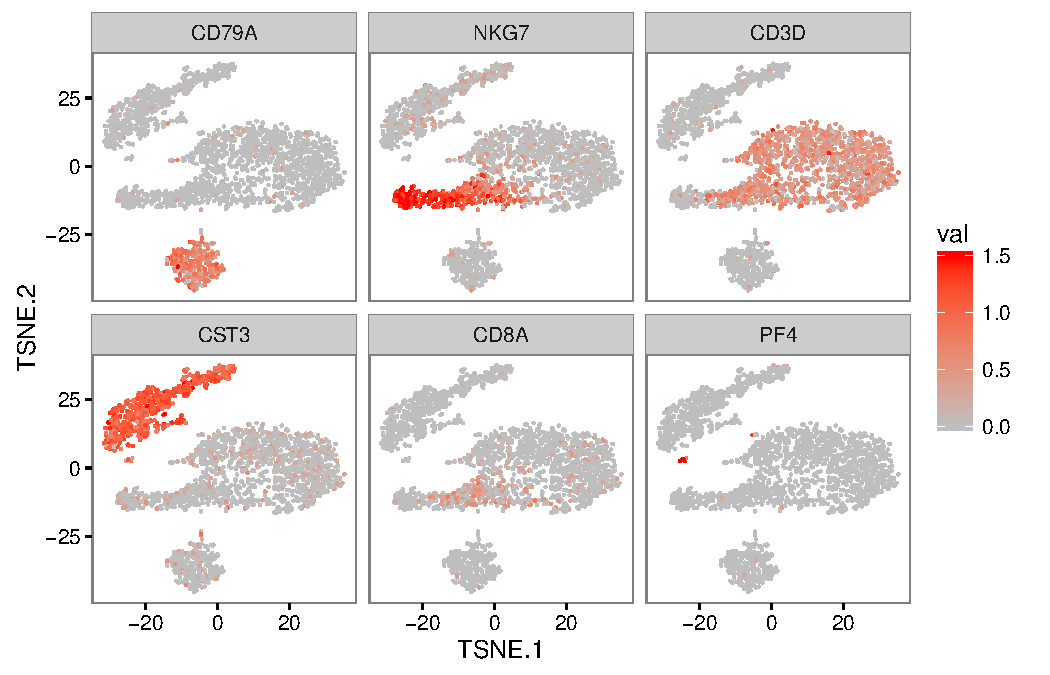
\includegraphics[width=\maxwidth]{figure/markers-1} 

}



\end{knitrout}
\caption{t-SNE projection where each cell is colored by normalized expression of the marker in the cell. Color scale represents the normalized expression of the marker. }
\label{fig:markers}
\end{center}
\end{figure}

\newpage
Because the input matrix \verb!gbm_log! is already normalized and log10-transformed, the color indicates the UMI counts for each gene under log10 scale (Figure \ref{fig:markers}). The specific gene markers already reveal cell types such as B cells, T cells, and natural killer (NK) cells. As expected, the cell-type-specific markers we have chosen are mostly unique to cells that are close together in the 2-D t-SNE projection.

\vspace{0.5in}
\section{Unbiased analysis using clustering results}
\subsection{Visualizing clustering results}
For some data sets, {\it de novo} cell-type discovery may be desired as prior knowledge of relevant marker genes can be limited or one may not want to introduce biases. In these cases it is useful to use unsupervised analysis to first algorithmically specify groupings of cells using the full data set. This can be achieved by applying any clustering methods on the loaded gene expression matrix \verb!exprs(gbm)! or the matrix in a reduced dimension space. In our implementation, for instance, we apply k-means clustering on the top 10 principle components of the gene expression matrix (after log-transformation, centering and scaling).

Because k-means clustering requires a specified number of clusters in the data set but the number of clusters in a data set may not be known {\it a priori}, it is helpful to consider multiple values of $k$. The output data from Cell Ranger\tm includes the pre-computed cluster labels sweeping $k$ from 2 to 10. So you can quickly visualize results for different values of $k$ and pick the one that agrees with your intuition (Figure \ref{fig:kmeans}). Here each cell is colored by its cluster ID.
\newpage
\begin{figure}[htbp]
\begin{center}
\begin{knitrout}
\definecolor{shadecolor}{rgb}{0.969, 0.969, 0.969}\color{fgcolor}\begin{kframe}
\begin{alltt}
\hlstd{n_clu} \hlkwb{<-} \hlnum{2}\hlopt{:}\hlnum{10}
\hlstd{km_res} \hlkwb{<-} \hlstd{analysis_results}\hlopt{$}\hlstd{kmeans} \hlcom{# load pre-computed kmeans results}
\hlstd{clu_res} \hlkwb{<-} \hlkwd{sapply}\hlstd{(n_clu,} \hlkwa{function}\hlstd{(}\hlkwc{x}\hlstd{) km_res[[}\hlkwd{paste}\hlstd{(x,}\hlstr{"clusters"}\hlstd{,}\hlkwc{sep}\hlstd{=}\hlstr{"_"}\hlstd{)]]}\hlopt{$}\hlstd{Cluster)}
\hlkwd{colnames}\hlstd{(clu_res)} \hlkwb{<-} \hlkwd{sapply}\hlstd{(n_clu,} \hlkwa{function}\hlstd{(}\hlkwc{x}\hlstd{)} \hlkwd{paste}\hlstd{(}\hlstr{"kmeans"}\hlstd{,x,}\hlkwc{sep}\hlstd{=}\hlstr{"."}\hlstd{))}
\hlkwd{visualize_clusters}\hlstd{(clu_res,tsne_proj[}\hlkwd{c}\hlstd{(}\hlstr{"TSNE.1"}\hlstd{,}\hlstr{"TSNE.2"}\hlstd{)])}
\end{alltt}
\end{kframe}

{\centering 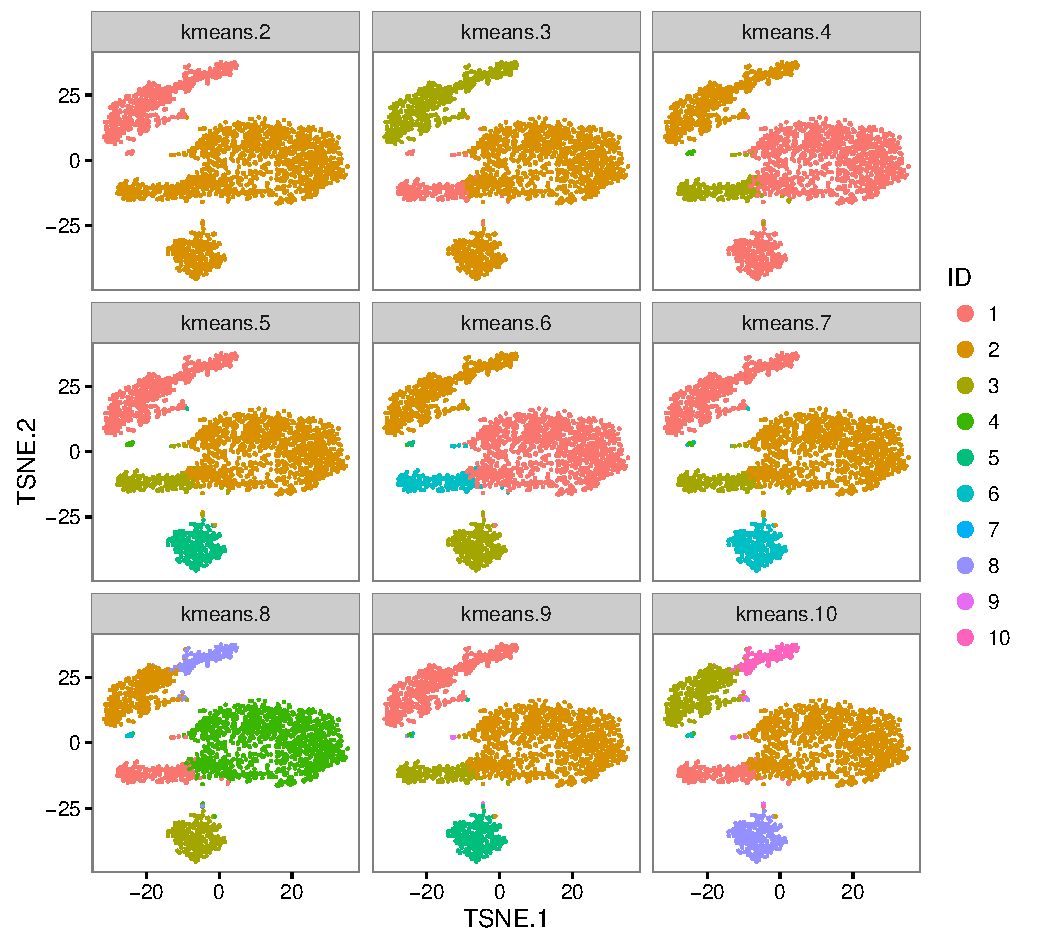
\includegraphics[width=\maxwidth]{figure/kmeans-1} 

}



\end{knitrout}
\caption{t-SNE projection where each cell is colored by cluster assigned by kmeans clustering. ID on the right represents the cluster ID.}
\label{fig:kmeans}
\end{center}
\end{figure}

\subsection{Analyzing cluster specific genes}
Using these integer cluster labels (or integer labels generated by any clustering algorithm), you can now perform differential gene analysis to identify gene markers that are specific to a particular cell population. For this example, we focus on the k-means clustering result above with 5 clusters (Figure \ref{fig:kmeans5}). Standard statistical tests can be applied to identify which genes are most differentially expressed across different cell types.
\newpage
\vspace{0.5in}
\begin{figure}[htbp]
\begin{center}
\begin{knitrout}
\definecolor{shadecolor}{rgb}{0.969, 0.969, 0.969}\color{fgcolor}\begin{kframe}
\begin{alltt}
\hlstd{example_K} \hlkwb{<-} \hlnum{5}    \hlcom{# number of clusters (use "Set3" for brewer.pal below if example_K > 8)}
\hlstd{example_col} \hlkwb{<-} \hlkwd{rev}\hlstd{(}\hlkwd{brewer.pal}\hlstd{(example_K,}\hlstr{"Set2"}\hlstd{))} \hlcom{# customize plotting colors}
\hlstd{cluster_result} \hlkwb{<-} \hlstd{analysis_results}\hlopt{$}\hlstd{kmeans[[}\hlkwd{paste}\hlstd{(example_K,}\hlstr{"clusters"}\hlstd{,}\hlkwc{sep}\hlstd{=}\hlstr{"_"}\hlstd{)]]}
\hlkwd{visualize_clusters}\hlstd{(cluster_result}\hlopt{$}\hlstd{Cluster,tsne_proj[}\hlkwd{c}\hlstd{(}\hlstr{"TSNE.1"}\hlstd{,}\hlstr{"TSNE.2"}\hlstd{)],}\hlkwc{colour}\hlstd{=example_col)}
\end{alltt}
\end{kframe}

{\centering 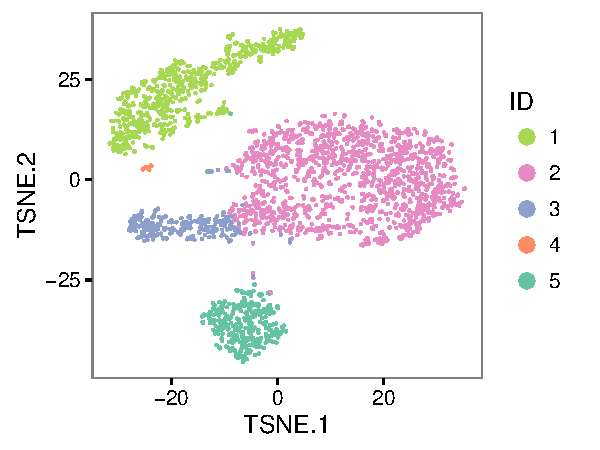
\includegraphics[width=\maxwidth]{figure/kmeans5-1} 

}



\end{knitrout}
\caption{t-SNE projection where each cell is colored by cluster assigned by kmeans clustering. ID on the right represents the cluster ID.}
\label{fig:kmeans5}
\end{center}
\end{figure}
You can compare the mean expression between a class of cells and the remaining ones, and then prioritize genes by how highly expressed they are in the class of interest. The function \verb!prioritize_top_genes! identifies markers that are up-regulated in particular clusters of cells. Note that there are many other ways to identify cluster-specific genes. The approach used here is quick when looking for cluster-specific genes among $\sim 20$k candidate genes.
\begin{knitrout}
\definecolor{shadecolor}{rgb}{0.969, 0.969, 0.969}\color{fgcolor}\begin{kframe}
\begin{alltt}
\hlcom{# sort the cells by the cluster labels}
\hlstd{cells_to_plot} \hlkwb{<-} \hlkwd{order_cell_by_clusters}\hlstd{(gbm, cluster_result}\hlopt{$}\hlstd{Cluster)}
\hlcom{# order the genes from most up-regulated to most down-regulated in each cluster}
\hlstd{prioritized_genes} \hlkwb{<-} \hlkwd{prioritize_top_genes}\hlstd{(gbm, cluster_result}\hlopt{$}\hlstd{Cluster,} \hlstr{"sseq"}\hlstd{,} \hlkwc{min_mean}\hlstd{=}\hlnum{0.5}\hlstd{)}
\end{alltt}
\begin{verbatim}
## Computing differential expression parameters...
## Comparing Cluster 1 against the other clusters...
## Comparing Cluster 2 against the other clusters...
## Comparing Cluster 3 against the other clusters...
## Comparing Cluster 4 against the other clusters...
## Comparing Cluster 5 against the other clusters...
\end{verbatim}
\end{kframe}
\end{knitrout}
Now that the genes for each cell type are prioritized, you can output the top genes specific to each cluster to a local folder. In this case, we output all the top 10 gene symbols for the 5 clusters to file.
\begin{knitrout}
\definecolor{shadecolor}{rgb}{0.969, 0.969, 0.969}\color{fgcolor}\begin{kframe}
\begin{alltt}
\hlstd{output_folder} \hlkwb{<-}\hlstr{"/path_to_your_local_folder/pbmc_data_public/pbmc3k/gene_sets"}
\hlkwd{write_cluster_specific_genes}\hlstd{(prioritized_genes, output_folder,} \hlkwc{n_genes}\hlstd{=}\hlnum{10}\hlstd{)}
\end{alltt}
\end{kframe}
\end{knitrout}
In addition, you can use the prioritized genes to plot a heat-map where the top three most up-regulated genes in each cluster are displayed. In addition, you can order the cells according to the cell IDs produced by k-means clustering to make the cell population signatures more apparent (Figure \ref{fig:heatmap}).
\begin{figure}[htbp]
\begin{center}
\begin{knitrout}
\definecolor{shadecolor}{rgb}{0.969, 0.969, 0.969}\color{fgcolor}\begin{kframe}
\begin{alltt}
\hlcom{# create values and axis annotations for pheatmap}
\hlkwd{gbm_pheatmap}\hlstd{(}\hlkwd{log_gene_bc_matrix}\hlstd{(gbm), prioritized_genes, cells_to_plot,}
             \hlkwc{n_genes}\hlstd{=}\hlnum{3}\hlstd{,} \hlkwc{colour}\hlstd{=example_col,} \hlkwc{limits}\hlstd{=}\hlkwd{c}\hlstd{(}\hlopt{-}\hlnum{1}\hlstd{,}\hlnum{2}\hlstd{))}
\end{alltt}
\end{kframe}

{\centering 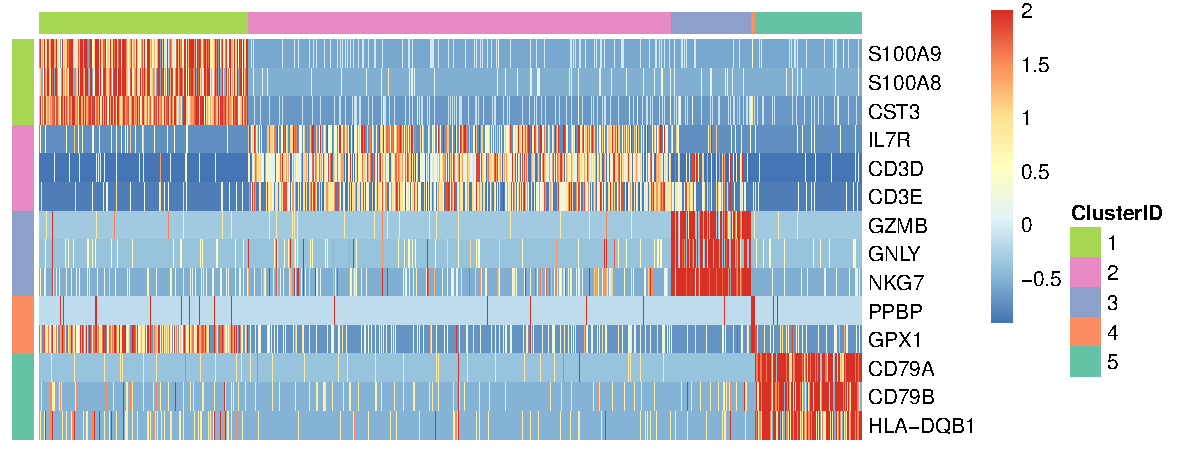
\includegraphics[width=\maxwidth]{figure/heatmap-1} 

}



\end{knitrout}
\caption{Heatmap of scaled expression of top 3 genes (row) in each cell (column). The horizontal and vertical bars around the heat map represents cluster ID assigned by kmeans clustering. Color scale represents scaled expression of the gene.}
\label{fig:heatmap}
\end{center}
\end{figure}

\newpage
Notice that the top three genes for each cluster already give us an idea on the identity of each cluster. For instance,
\begin{itemize}
\item
S100A9 is among the top 3 most expressed genes in Cluster 1, suggesting a population of monocytes;
\item
CD3D is among the top 3 most expressed genes in Cluster 2, suggesting a population of T cells;
\item
NKG7 is among the top 3 most expressed genes in Cluster 3, suggesting a population of NK cells;
\item
PPBP is among the top 3 most expressed genes in Cluster 4, suggesting a population of megakaryocytes;
\item
CD79A is among the top 3 most expressed genes in Cluster 5, suggesting a population of B cells.
\end{itemize}

You can also find out the size of each cluster. For example, about 13\% cells were classified as B cells in this sample.

\begin{knitrout}
\definecolor{shadecolor}{rgb}{0.969, 0.969, 0.969}\color{fgcolor}\begin{kframe}
\begin{alltt}
\hlkwd{cell_composition}\hlstd{(cluster_result}\hlopt{$}\hlstd{Cluster,}
                 \hlkwc{anno}\hlstd{=}\hlkwd{c}\hlstd{(}\hlstr{"monocytes"}\hlstd{,}\hlstr{"T cells"}\hlstd{,}\hlstr{"NK cells"}\hlstd{,}\hlstr{"megakaryocytes"}\hlstd{,}\hlstr{"B cells"}\hlstd{))}
\end{alltt}
\begin{verbatim}
## Cell composition:
##            1           2         3          4                5        
## annotation "monocytes" "T cells" "NK cells" "megakaryocytes" "B cells"
## num_cells  "685"       "1391"    "264"      "12"             "348"    
## proportion "0.2537"    "0.51519" "0.09778"  "0.00444"        "0.12889"
\end{verbatim}
\end{kframe}
\end{knitrout}
\vspace{0.5in}
\section{Analyzing multiple data sets}
\subsection{Merging multiple pbmc data sets}

{\color{Red}Note: the following section is deprecated. As of cellranger 1.2.0, you can use the \verb!cellranger aggr! pipeline, which combines matrices and performs read-depth normalization for you. The \verb!equalize_gbms! and \verb!load_molecule_info! functions are no longer officially supported.}

It is very common to pool data from different lanes of a 10x run or even different samples when analyzing single cell data sets. Because the output of these experiments will involve multiple Cell Ranger runs (one per Cell Ranger run), the pre-computed information such as t-SNE projections and k-means clustering need to be re-computed after pooling different data sets.
Here we demonstrate how to merge two PBMC data sets where 2 libraries (pbmc3k and pbmc6k) were made and sequenced on different sequencers. You can download the data and store them in the format as you did for the single PBMC example and specify the path for each sample.
\begin{knitrout}
\definecolor{shadecolor}{rgb}{0.969, 0.969, 0.969}\color{fgcolor}\begin{kframe}
\begin{alltt}
\hlstd{cellranger_pipestance_path_1} \hlkwb{<-} \hlstr{"/path/to/your/pipeline/output/directory1"}
\hlstd{cellranger_pipestance_path_2} \hlkwb{<-} \hlstr{"/path/to/your/pipeline/output/directory2"}
\hlstd{gbm1} \hlkwb{<-} \hlkwd{load_cellranger_matrix}\hlstd{(cellranger_pipestance_path_1)}
\hlstd{gbm2} \hlkwb{<-} \hlkwd{load_cellranger_matrix}\hlstd{(cellranger_pipestance_path_2)}
\end{alltt}
\end{kframe}
\end{knitrout}
Alternatively, you can download the two datasets using the \verb!download_sample! function. Notice that you will need to set the option \verb!lite=FALSE! to download necessary molecule information in order to merge multiple data sets. The additional molecule information file can be a few hundred megabytes, and hence downloading the sample will take longer.
\begin{knitrout}
\definecolor{shadecolor}{rgb}{0.969, 0.969, 0.969}\color{fgcolor}\begin{kframe}
\begin{alltt}
\hlstd{host} \hlkwb{<-} \hlstr{"https://s3-us-west-2.amazonaws.com/10x.files/samples/cell/"}
\hlstd{pipestance_path_1} \hlkwb{<-} \hlstr{"/path/to/your/local/directory/for/pbmc6k"}
\hlstd{pipestance_path_2} \hlkwb{<-} \hlstr{"/path/to/your/local/directory/for/pbmc3k"}
\hlkwd{download_sample}\hlstd{(}\hlstr{"pbmc6k"}\hlstd{,pipestance_path_1,host,}\hlkwc{lite}\hlstd{=}\hlnum{FALSE}\hlstd{)}
\hlkwd{download_sample}\hlstd{(}\hlstr{"pbmc3k"}\hlstd{,pipestance_path_2,host,}\hlkwc{lite}\hlstd{=}\hlnum{FALSE}\hlstd{)}
\hlstd{gbm1} \hlkwb{<-} \hlkwd{load_cellranger_matrix}\hlstd{(pipestance_path_1)}
\hlstd{gbm2} \hlkwb{<-} \hlkwd{load_cellranger_matrix}\hlstd{(pipestance_path_2)}
\end{alltt}
\end{kframe}
\end{knitrout}


To merge multiple data sets, you can simply merge multiple \verb!gbm! objects and re-normalize using the function: \verb!concatenate_gene_bc_matrices!. However, we recommend equalizing read depths between samples before merging to reduce the batch effect that might have been introduced through sequencing. You can use \verb!equalize_gbm! to sub-sample a list of \verb!gbm! objects to generate new data sets with depth equal to that of the sample with the least reads. You can also apply any other batch effect removal strategy on this list of \verb!gbm! objects to account for the differences across gene expression matrices in your study design. The cell pipestance indices are stored as batch labels using \verb!merged_ID!.
\begin{knitrout}
\definecolor{shadecolor}{rgb}{0.969, 0.969, 0.969}\color{fgcolor}\begin{kframe}
\begin{alltt}
\hlkwd{set.seed}\hlstd{(}\hlnum{0}\hlstd{)}
\hlstd{gbm_list} \hlkwb{<-} \hlkwd{list}\hlstd{(gbm1, gbm2)}
\hlstd{gbm_list} \hlkwb{<-} \hlkwd{lapply}\hlstd{(gbm_list,load_molecule_info)} \hlcom{# load sample molecule information}
\hlstd{gbm_list_equalized} \hlkwb{<-} \hlkwd{equalize_gbms}\hlstd{(gbm_list)}   \hlcom{# equalize the gene-barcode matrices}
\hlstd{merged_gbm} \hlkwb{<-} \hlkwd{concatenate_gene_bc_matrices}\hlstd{(gbm_list_equalized)}
\hlstd{merged_ID} \hlkwb{<-} \hlkwd{unlist}\hlstd{(}\hlkwd{lapply}\hlstd{(}\hlnum{1}\hlopt{:}\hlkwd{length}\hlstd{(gbm_list),} \hlkwa{function}\hlstd{(}\hlkwc{x}\hlstd{)} \hlkwd{rep}\hlstd{(x,}\hlkwd{dim}\hlstd{(gbm_list[[x]])[}\hlnum{2}\hlstd{])))}
\end{alltt}
\end{kframe}
\end{knitrout}
\subsection{Re-running PCA, t-SNE and k-means clustering}
When two different samples are merged, you need to recompute the the PCA dimension reduction, t-SNE projection, and k-means clustering (or other methods of your choice).
\begin{knitrout}
\definecolor{shadecolor}{rgb}{0.969, 0.969, 0.969}\color{fgcolor}\begin{kframe}
\begin{alltt}
\hlkwd{set.seed}\hlstd{(}\hlnum{0}\hlstd{)}
\hlstd{n_clust} \hlkwb{<-} \hlnum{5}
\hlstd{pca_result} \hlkwb{<-} \hlkwd{run_pca}\hlstd{(merged_gbm)}
\hlstd{tsne_result} \hlkwb{<-} \hlkwd{run_tsne}\hlstd{(pca_result)}
\hlstd{kmeans_result} \hlkwb{<-} \hlkwd{run_kmeans_clustering}\hlstd{(pca_result,}\hlkwc{k}\hlstd{=n_clust)}
\hlcom{# included re-named cell IDs, t-SNE and k-means result in a merged data frame}
\hlstd{merged_tsne_clust} \hlkwb{<-} \hlkwd{data.frame}\hlstd{(}\hlkwc{Barcode}\hlstd{=}\hlkwd{as.factor}\hlstd{(}\hlnum{1}\hlopt{:}\hlstd{tsne_result}\hlopt{$}\hlstd{N),}
                                \hlkwc{TSNE.1}\hlstd{=tsne_result}\hlopt{$}\hlstd{Y[,}\hlnum{1}\hlstd{],}\hlkwc{TSNE.2}\hlstd{=tsne_result}\hlopt{$}\hlstd{Y[,}\hlnum{2}\hlstd{],}
                                \hlkwc{Cluster}\hlstd{=kmeans_result}\hlopt{$}\hlstd{cluster,}\hlkwc{Batch}\hlstd{=merged_ID)}
\end{alltt}
\end{kframe}
\end{knitrout}

To further investigate potential batch effects in the data, we recommend coloring the same projection by batch labels (Figure \ref{fig:tsne_batch}). This is because clustering results can sometimes reflect technical effects depending on the nature of the study. In our case, the two samples consist of healthy PBMCs from the same donor, and the two batches are well-mixed in the data. In other cases where the batches are not limited to technical effects, it is reasonable to see some cell populations seperated by batches.
\newpage
\begin{figure}[htbp]
\begin{center}
\begin{knitrout}
\definecolor{shadecolor}{rgb}{0.969, 0.969, 0.969}\color{fgcolor}\begin{kframe}
\begin{alltt}
\hlstd{p_c} \hlkwb{<-} \hlkwd{visualize_clusters}\hlstd{(merged_tsne_clust}\hlopt{$}\hlstd{Cluster,merged_tsne_clust[}\hlkwd{c}\hlstd{(}\hlstr{"TSNE.1"}\hlstd{,}\hlstr{"TSNE.2"}\hlstd{)],}
       \hlkwc{title}\hlstd{=}\hlstr{"k-means clustering labels"}\hlstd{)}
\hlstd{p_b} \hlkwb{<-} \hlkwd{visualize_clusters}\hlstd{(merged_tsne_clust}\hlopt{$}\hlstd{Batch,merged_tsne_clust[}\hlkwd{c}\hlstd{(}\hlstr{"TSNE.1"}\hlstd{,}\hlstr{"TSNE.2"}\hlstd{)],}
       \hlkwc{title}\hlstd{=}\hlstr{"batch labels"}\hlstd{)}
\hlkwd{multiplot}\hlstd{(p_c, p_b,} \hlkwc{cols}\hlstd{=}\hlnum{2}\hlstd{)}
\end{alltt}
\end{kframe}

{\centering 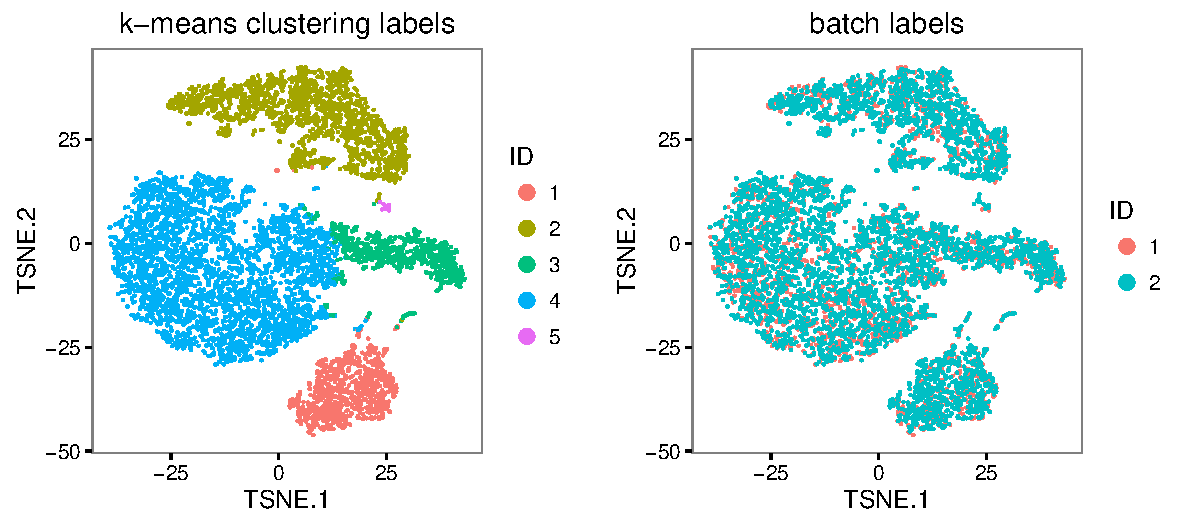
\includegraphics[width=\maxwidth]{figure/plot_tsne_batch-1} 

}



\end{knitrout}
\caption{t-SNE projection where (Left) each cell is colored by cluster assigned in kmeans clustering, (Right) each cell is colored by sample ID, where 1 represents pbmc3k, and 2 represents pbmc6k.}
\label{fig:tsne_batch}
\end{center}
\end{figure}

Finally, you can repeat the analysis shown in the previous section on \verb!merged_gbm! to identify cluster specific genes from the new clustering result.

\section{Subsetting the matrix by cell or gene}
You can select submatrices of the matrix either by cell or by gene as if it were a standard matrix in R. The first dimension (rows) consists of genes and the second dimension (columns) consists of cell-barcodes.

\begin{knitrout}
\definecolor{shadecolor}{rgb}{0.969, 0.969, 0.969}\color{fgcolor}\begin{kframe}
\begin{alltt}
\hlstd{subset_by_cell} \hlkwb{<-} \hlstd{gbm[,}\hlkwd{c}\hlstd{(}\hlstr{"AAACATACAACCAC-1"}\hlstd{,} \hlstr{"AAACATTGAGCTAC-1"}\hlstd{)]}
\hlstd{subset_by_gene_id} \hlkwb{<-} \hlstd{gbm[}\hlstr{"ENSG00000167286"}\hlstd{,]}
\hlstd{subset_by_gene_symbol} \hlkwb{<-} \hlstd{gbm[}\hlkwd{which}\hlstd{(}\hlkwd{fData}\hlstd{(gbm)}\hlopt{$}\hlstd{symbol} \hlopt{==} \hlstr{'CD3D'}\hlstd{),]}
\hlstd{subset_by_cell_and_gene} \hlkwb{<-} \hlstd{gbm[}\hlstr{"ENSG00000167286"}\hlstd{,} \hlkwd{c}\hlstd{(}\hlstr{"AAACATACAACCAC-1"}\hlstd{,} \hlstr{"AAACATTGAGCTAC-1"}\hlstd{)]}

\hlcom{# You can then use the exprs, fData and pData functions on this subsetted object}
\hlkwd{table}\hlstd{(}\hlkwd{exprs}\hlstd{(subset_by_gene_symbol)[}\hlnum{1}\hlstd{,])}
\end{alltt}
\begin{verbatim}
## 
##    0    1    2    3    4    5    6    7    8    9   10   11   12   15   24 
## 1295  422  338  273  155   98   51   34   11    6    7    2    2    1    1 
##   27   29   36   40 
##    1    1    1    1
\end{verbatim}
\end{kframe}
\end{knitrout}

\section{Session Info}
\begin{knitrout}
\definecolor{shadecolor}{rgb}{0.969, 0.969, 0.969}\color{fgcolor}\begin{kframe}
\begin{alltt}
\hlkwd{sessionInfo}\hlstd{()}
\end{alltt}
\begin{verbatim}
## R version 3.1.1 (2014-07-10)
## Platform: x86_64-pc-linux-gnu (64-bit)
## 
## locale:
##  [1] LC_CTYPE=en_US.UTF-8       LC_NUMERIC=C              
##  [3] LC_TIME=en_US.UTF-8        LC_COLLATE=en_US.UTF-8    
##  [5] LC_MONETARY=en_US.UTF-8    LC_MESSAGES=en_US.UTF-8   
##  [7] LC_PAPER=en_US.UTF-8       LC_NAME=C                 
##  [9] LC_ADDRESS=C               LC_TELEPHONE=C            
## [11] LC_MEASUREMENT=en_US.UTF-8 LC_IDENTIFICATION=C       
## 
## attached base packages:
## [1] parallel  methods   stats     graphics  grDevices utils     datasets 
## [8] base     
## 
## other attached packages:
##  [1] cellrangerRkit_1.1.0 Rmisc_1.5            plyr_1.8.3          
##  [4] lattice_0.20-31      bit64_0.9-5          bit_1.1-12          
##  [7] ggplot2_2.1.0        RColorBrewer_1.1-2   Biobase_2.26.0      
## [10] BiocGenerics_0.12.1  Matrix_1.2-1         knitr_1.12.3        
## 
## loaded via a namespace (and not attached):
##  [1] chron_2.3-47     colorspace_1.2-6 data.table_1.9.6 digest_0.6.10   
##  [5] evaluate_0.8.3   formatR_1.3      grid_3.1.1       gtable_0.2.0    
##  [9] highr_0.5.1      irlba_2.0.0      labeling_0.3     magrittr_1.5    
## [13] munsell_0.4.3    pheatmap_1.0.8   Rcpp_0.12.3      reshape2_1.4.1  
## [17] rhdf5_2.16.0     Rtsne_0.11       scales_0.3.0     stringi_1.0-1   
## [21] stringr_1.1.0    tools_3.1.1      zlibbioc_1.12.0
\end{verbatim}
\end{kframe}
\end{knitrout}

\bibliographystyle{unsrt}
\bibliography{cellrangerrkit-bib}

\end{document}
